\documentclass[11pt,border=5pt]{standalone}
\usepackage[T1]{fontenc}
\usepackage{lmodern}
\IfFileExists{Jost.sty}{\usepackage{Jost}}{}
\usepackage{pgfplots}
\pgfplotsset{compat=1.18}
\usepackage{xcolor}

\definecolor{teal}{HTML}{004D40}
\definecolor{coral}{HTML}{FF655D}
\definecolor{yellow}{HTML}{F1DB4B}
\definecolor{lightgray}{HTML}{D0D0D0}
\definecolor{refgray}{HTML}{AAAAAA}

\begin{document}
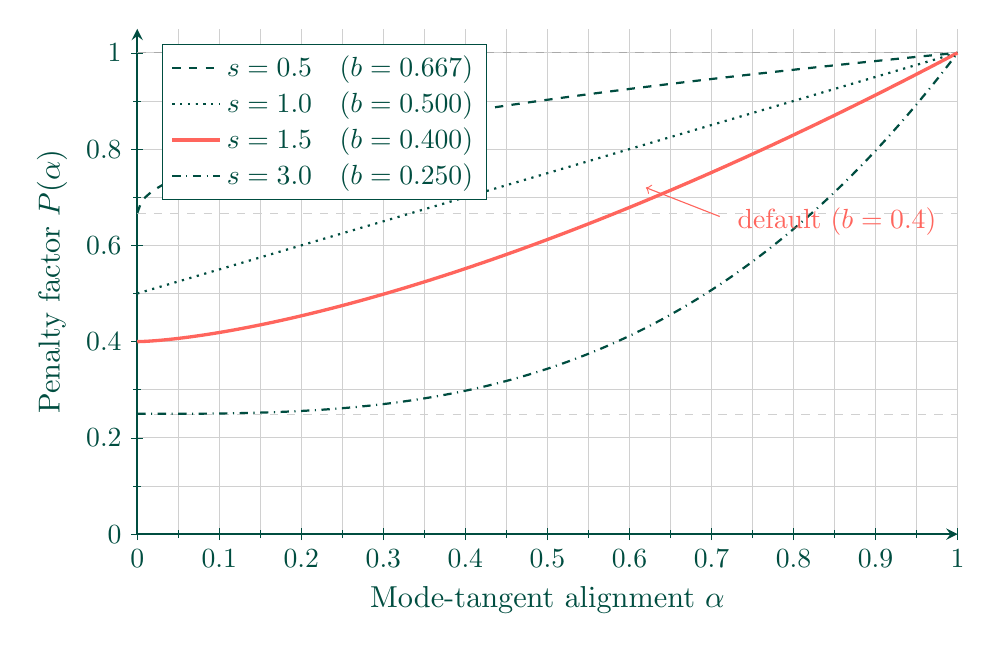
\begin{tikzpicture}
\begin{axis}[
    width=12cm,
    height=8cm,
    domain=0:1,
    samples=200,
    xmin=0, xmax=1,
    ymin=0, ymax=1.05,
    xlabel={Mode-tangent alignment $\alpha$},
    ylabel={Penalty factor $P(\alpha)$},
    xlabel style={font=\fontsize{11}{13}\selectfont, text=teal},
    ylabel style={font=\fontsize{11}{13}\selectfont, text=teal},
    tick label style={font=\fontsize{10}{12}\selectfont, text=teal},
    axis lines=left,
    axis line style={teal, thick},
    tick style={teal},
    minor grid style={lightgray, very thin},
    major grid style={lightgray, thin},
    grid=both,
    minor tick num=1,
    legend style={
      at={(0.03,0.97)},
      anchor=north west,
      font=\fontsize{10}{12}\selectfont,
      draw=teal,
      fill=white,
      text=teal,
    },
    clip=false,
  ]

  % Reference line at P=1
  \addplot[refgray, dashed, thin, forget plot]
    coordinates {(0,1) (1,1)};

  % Base value lines (very light)
  % s=0.5: b=0.667
  \addplot[lightgray, dashed, very thin, forget plot]
    coordinates {(0,0.667) (1,0.667)};
  % s=1.0: b=0.500
  \addplot[lightgray, dashed, very thin, forget plot]
    coordinates {(0,0.500) (1,0.500)};
  % s=1.5: b=0.400
  \addplot[lightgray, dashed, very thin, forget plot]
    coordinates {(0,0.400) (1,0.400)};
  % s=3.0: b=0.250
  \addplot[lightgray, dashed, very thin, forget plot]
    coordinates {(0,0.250) (1,0.250)};

  % s=0.5, b = 1/(1+0.5) = 0.667
  \addplot[teal, dashed, thick]
    {0.667 + (1-0.667)*x^0.5};
  \addlegendentry{$s = 0.5$\quad$(b = 0.667)$}

  % s=1.0, b = 1/(1+1) = 0.500
  \addplot[teal, dotted, thick]
    {0.500 + (1-0.500)*x^1.0};
  \addlegendentry{$s = 1.0$\quad$(b = 0.500)$}

  % s=1.5, b = 1/(1+1.5) = 0.400 -- highlighted as default
  \addplot[coral, solid, very thick]
    {0.400 + (1-0.400)*x^1.5};
  \addlegendentry{$s = 1.5$\quad$(b = 0.400)$}

  % s=3.0, b = 1/(1+3) = 0.250
  \addplot[teal, dash dot, thick]
    {0.250 + (1-0.250)*x^3.0};
  \addlegendentry{$s = 3.0$\quad$(b = 0.250)$}

  % Annotation for s=1.5
  \node[font=\fontsize{10}{12}\selectfont, text=coral, anchor=west]
    at (axis cs:0.72,0.65) {default $(b = 0.4)$};
  \draw[->, coral, thin] (axis cs:0.71,0.66) -- (axis cs:0.62,0.72);

\end{axis}
\end{tikzpicture}
\end{document}
